\documentclass[11pt,a4paper]{article}

\usepackage[margin=1in]{geometry}
\usepackage[T1]{fontenc}
\usepackage[utf8]{inputenc}
\usepackage{lmodern}
\usepackage{microtype}
\usepackage{setspace}
\usepackage{booktabs}
\usepackage{graphicx}
\usepackage{tikz}
\usetikzlibrary{arrows.meta,positioning}
\usepackage{amsmath,amssymb}
\usepackage{enumitem}
\usepackage{xcolor}
\usepackage{caption}
\usepackage{subcaption}
\usepackage[section]{placeins}
\usepackage{flafter}
\usepackage{hyperref}

\hypersetup{
  colorlinks=true,
  linkcolor=black,
  citecolor=black,
  urlcolor=black
}

\definecolor{headerblue}{RGB}{20,55,95}

\setstretch{1.18}
\setlength{\parskip}{0.4em}
\setlength{\parindent}{1.2em}

\begin{document}

% ===========================================================================
% Page 1 --- title page only (no abstract, no body text)
% ===========================================================================
\begin{titlepage}
\hypersetup{pageanchor=false}
\thispagestyle{empty}
\centering

\vspace*{1.6cm}

{\large 22AIE301 \textperiodcentered\ Probability and Reasoning}

\vspace{2.4cm}

{\LARGE\bfseries Probabilistic Topic Modeling for\\[0.3em]
Research Trend Analysis}

\vspace{0.7cm}

{\Large A Hybrid LDA--LLM Approach}

\vspace{2.2cm}

{\large A Project Report}

\vspace{0.35cm}

{\normalsize submitted in partial fulfilment of the requirements\\
of the course 22AIE301}

\vspace{1.8cm}

{\normalsize Submitted by}

\vspace{0.35cm}

{\Large\textbf{Kaushik}}

\vfill

{\normalsize August 2026}

\vspace{1.4cm}

{\small Based on Paul et al., \emph{IAENG International Journal of Computer Science}, 52(2), 2025,\\
and George \& Sumathy, \emph{International Journal of Information Technology}, 15, 2023.}

\vspace{0.8cm}
\end{titlepage}

% ===========================================================================
% Page 2 onwards --- main matter
% ===========================================================================
\hypersetup{pageanchor=true}
\pagenumbering{arabic}

\begin{abstract}
\noindent
The rate at which papers appear in machine learning makes a purely manual literature survey impractical. Topic models are one way to compress a corpus into a small set of themes that can be inspected, tracked across years, and used to retrieve related work. Latent Dirichlet Allocation (LDA) is still a natural choice for this task because it is a generative model: a document is a mixture of topics and a topic is a distribution over words. The same property that makes LDA easy to interpret, however, is also its main restriction. The model sees only co-occurrence. Terms that never share a document, even when they are close in meaning, do not help one another, and the resulting topics can look statistically tidy while remaining hard to read.

This report keeps LDA as the probabilistic component and adds a frozen Sentence-BERT encoder as a second view of each document. The two representations are concatenated with a scalar weight $\alpha$, reduced with UMAP, and clustered with $k$-means. Cluster labels are turned back into word lists with class-based TF-IDF, so that the hybrid can be scored with the same coherence measures as LDA. The comparison requested for the course is therefore direct: $C_v$, NPMI and UMass for baseline LDA against the same scores for the hybrid. On 20~Newsgroups the best hybrid $C_v$ is $0.79$, against $0.51$ for LDA. On a year-stratified sample of arXiv abstracts from 2018--2025 the corresponding figures are $0.57$ at $\alpha=0.5$ and $0.72$ after selecting $\alpha$ on the coherence curve, against $0.44$ for LDA. The same pipeline also produces a yearly plot of topic prevalence and a small related-work search over document embeddings.
\end{abstract}

\section{Introduction}
\label{sec:intro}

Topic models are used here for a limited purpose. Given a collection of abstracts, we would like a short list of themes, a sense of how those themes change from year to year, and a way to find papers that sit near a query. LDA~\cite{blei2003} remains a reasonable starting point because inference returns two objects that are easy to explain in a probability course. The document-topic vector $\theta_d$ says how much of document $d$ is assigned to each topic. The topic-word vector $\phi_k$ says which terms characterise topic $k$. Both are distributions, so they can be averaged over publication years or treated as a soft assignment when a new abstract arrives.

The cost of that simplicity is well known. LDA treats a document as a bag of words. It does not see word order, and it has no notion that \emph{transformer} and \emph{self-attention} are related unless those terms happen to co-occur often enough in the training set. Contextual embeddings make the opposite trade-off. Models such as BERT~\cite{devlin2019} and Sentence-BERT~\cite{reimers2019} place semantically similar sentences near one another even when their surface forms differ. Clustering those vectors often produces tighter groups than LDA, but it does not, by itself, give a generative topic distribution $p(z\mid d)$.

A practical compromise, used by Paul et al.~\cite{paul2025} and by George and Sumathy~\cite{george2023}, is to concatenate the two representations and cluster the result. Paul et al.\ evaluate the combination with topic coherence on news text and on 20~Newsgroups. George and Sumathy reduce the concatenated vectors with PCA, t-SNE or UMAP, run $k$-means, and report silhouette scores on CORD-19. The present project follows that design, with three changes that matter for a scientific corpus. The comparison against LDA is made with $C_v$ (and NPMI, UMass), not only with silhouette. The concatenation weight $\alpha$ is treated as a parameter and chosen on the coherence curve rather than fixed in advance. Publication years are retained so that mean $\theta$ can be plotted over time, and a small dashboard is provided for inspecting topics and retrieving related abstracts.

Section~\ref{sec:related} places the method against the two source papers and the coherence literature. Section~\ref{sec:method} specifies preprocessing, LDA, embeddings, the hybrid vector, clustering, and the extra modules for trends and retrieval. Section~\ref{sec:impl} records where those pieces live in the code. Sections~\ref{sec:setup} and~\ref{sec:results} describe the experiments and the numbers. Section~\ref{sec:discuss} comments on why the hybrid helps, where it does not, and how the results sit next to prior work. Section~\ref{sec:end} concludes.

\section{Related work}
\label{sec:related}

Blei, Ng and Jordan~\cite{blei2003} introduced LDA as a three-level hierarchical Bayesian model over a corpus. Later variants add correlations among topics, supervision, or dynamics~\cite{blei2006}. The experiments here stay with vanilla LDA. The aim is not to replace the generative model, but to see whether a semantic embedding can improve the topics that LDA already produces.

On the embedding side, Sentence-BERT~\cite{reimers2019} fine-tunes BERT with a siamese objective so that cosine similarity between sentence vectors is meaningful. SciBERT~\cite{beltagy2019} is a closer match to scientific prose and is left as an optional encoder in the code. BERTopic~\cite{grootendorst2022} clusters document embeddings and names each cluster with class-based TF-IDF; that labelling step is adopted below for hybrid clusters.

Hybrid LDA--BERT models have appeared in several forms. Xie et al.~\cite{xie2020} use both signals for monolingual and multilingual topic similarity. Paul et al.~\cite{paul2025} concatenate BERT embeddings with LDA topic proportions and report a $C_v$ increase from $0.63$ to $0.66$ on their news collection. George and Sumathy~\cite{george2023} study the same concatenation followed by dimensionality reduction and $k$-means; UMAP with BERT--LDA gave the highest silhouette on CORD-19. What is missing from that pair of papers, relative to the brief for this project, is a $C_v$ comparison against LDA on scientific abstracts together with an explicit search over $\alpha$.

Topic coherence is the natural metric for that comparison. R\"oder, Both and Hinneburg~\cite{roder2015} examined a large family of coherence measures and found that $C_v$, which combines a sliding-window NPMI with an indirect cosine confirmation, agreed most closely with human judgements of topic quality. UMass and NPMI are reported as well, mainly as a check that the ranking of models does not depend on a single formula.

\section{Method}
\label{sec:method}

The pipeline is summarised in Figure~\ref{fig:pipeline}. After cleaning, two representations are computed from the same abstracts: an LDA topic vector and a Sentence-BERT embedding. They are concatenated, reduced, clustered, and scored.

\begin{figure}[htbp]
\centering
\resizebox{\textwidth}{!}{%
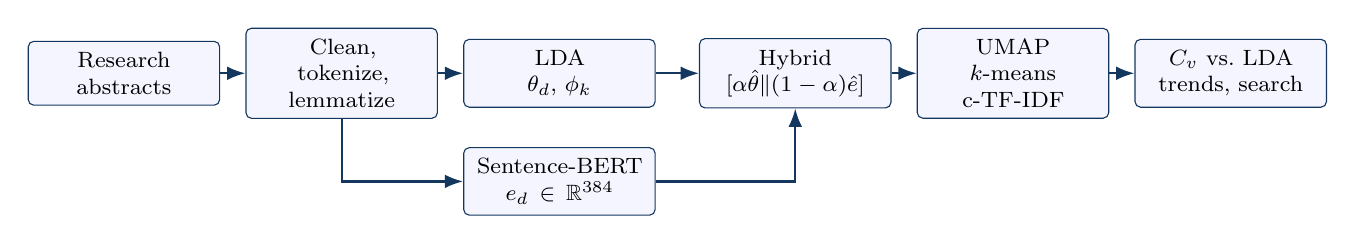
\begin{tikzpicture}[
  font=\footnotesize,
  box/.style={draw=headerblue, rounded corners=2pt, align=center, inner sep=4pt, fill=blue!4, text width=2.15cm},
  arr/.style={-{Latex}, thick, headerblue}
]
\node[box] (raw) {Research\\abstracts};
\node[box, right=0.32cm of raw] (prep) {Clean,\\tokenize,\\lemmatize};
\node[box, right=0.32cm of prep] (lda) {LDA\\$\theta_d$, $\phi_k$};
\node[box, below=0.5cm of lda] (emb) {Sentence-BERT\\$e_d\in\mathbb{R}^{384}$};
\node[box, right=0.55cm of lda] (hyb) {Hybrid\\$[\alpha\hat\theta \Vert (1-\alpha)\hat e]$};
\node[box, right=0.32cm of hyb] (umap) {UMAP\\$k$-means\\c-TF-IDF};
\node[box, right=0.32cm of umap] (eval) {$C_v$ vs.\ LDA\\trends, search};
\draw[arr] (raw) -- (prep);
\draw[arr] (prep) -- (lda);
\draw[arr] (prep.south) |- (emb.west);
\draw[arr] (lda) -- (hyb);
\draw[arr] (emb) -| (hyb.south);
\draw[arr] (hyb) -- (umap);
\draw[arr] (umap) -- (eval);
\end{tikzpicture}%
}
\caption{Processing pipeline. LDA and Sentence-BERT are computed from the same cleaned abstracts and combined before clustering.}
\label{fig:pipeline}
\end{figure}

\subsection{Preprocessing}
Each document is lowercased. URLs, email addresses and simple citation markers are removed, as are characters outside the English alphabet. A stopword list combining the NLTK English list with a few frequent scientific fillers (\texttt{method}, \texttt{result}, \texttt{paper}, and similar) is applied, after which tokens are lemmatized with WordNet. Documents that fall below eight tokens are dropped. The same token sequences are used to build the LDA dictionary and, later, the class-based TF-IDF counts.

\subsection{Baseline LDA}
Let $K$ be the number of topics. LDA represents document $d$ by a point on the simplex,
\begin{equation}
  \theta_d \in \Delta^{K-1}, \qquad \theta_{d,k} = p(z=k\mid d),
\end{equation}
and topic $k$ by a distribution $\phi_k = p(w\mid z=k)$ over the vocabulary. Training uses gensim with ten passes and automatic Dirichlet hyperparameters. The baseline topic for $k$ is the list of $N=10$ highest-probability words under $\phi_k$. Those lists are what $C_v$ is computed on for LDA.

\subsection{Sentence embeddings}
Each original abstract (not the bag-of-words version) is passed through a frozen Sentence-BERT encoder, \texttt{all-MiniLM-L6-v2}, giving a 384-dimensional vector $e_d$ that is then $\ell_2$-normalised. The encoder is not fine-tuned. Treating it as a fixed feature map is enough for the question asked here and keeps the experiments runnable on a laptop.

\subsection{Hybrid document vector}
Following~\cite{paul2025,george2023}, the two views are concatenated. Write $\hat\theta_d$ and $\hat e_d$ for the $\ell_2$-normalised LDA and embedding vectors. The hybrid representation is
\begin{equation}
\label{eq:hybrid}
  h_d = \big[\, \alpha\,\hat\theta_d \;\Vert\; (1-\alpha)\,\hat e_d \,\big].
\end{equation}
The scalar $\alpha\in[0,1]$ is the weight on the LDA view. At the endpoints, $\alpha=1$ uses only topic proportions and $\alpha=0$ uses only embeddings. Intermediate values keep both. In the experiments $\alpha$ is first set to $0.5$ and then swept over $\{0, 0.25, 0.5, 0.75, 1\}$ at the best $K$, retaining the value that maximises $C_v$.

\subsection{Reduction, clustering and cluster labels}
The vectors $h_d$ are reduced with UMAP~\cite{mcinnes2018} and partitioned with $k$-means into $K$ groups. PCA and t-SNE are run as well, mainly to reproduce the silhouette comparison in~\cite{george2023}. Because a cluster is a set of documents rather than a multinomial over words, topic words are recovered with class-based TF-IDF~\cite{grootendorst2022}: all tokens in a cluster are concatenated, term frequencies are computed, and each term is reweighted by a class-level inverse document frequency. The top ten terms of each cluster are then scored with the same coherence functions used for LDA. Scoring both models on word lists of the same form is what makes the $C_v$ comparison legitimate. If the hybrid were scored on a different kind of output, a higher number would not mean much.

\subsection{Coherence and auxiliary scores}
For a set of $K$ word lists, gensim's \texttt{CoherenceModel} supplies $C_v$, $C_{\mathrm{NPMI}}$ and $U_{\mathrm{Mass}}$. Topic diversity is the fraction of unique terms among the collected top words; low diversity is a sign that several topics have collapsed onto the same vocabulary. Silhouette is computed in the reduced space and is treated as a clustering diagnostic, not as a substitute for coherence.

\subsection{Prevalence over years}
When a publication year $y$ is available, the mean LDA assignment in that year is
\begin{equation}
  \bar\theta_{y,k}
  = \frac{1}{|\{d:\mathrm{year}(d)=y\}|}
    \sum_{d:\,\mathrm{year}(d)=y} \theta_{d,k}.
\end{equation}
Plotting $\bar\theta_{y,k}$ against $y$ is a crude but readable picture of how probability mass moves. It is not a dynamic topic model~\cite{blei2006}; the topics themselves are estimated once on the pooled corpus.

\subsection{Retrieving related work}
A query abstract is encoded to $e_q$ and, if an LDA model is in memory, mapped to $\theta_q$ by inference on its bag of words. Neighbouring corpus papers are retrieved by cosine similarity in the hybrid (or embedding) space. A soft topic ranking is obtained by blending $\theta_q$ with the similarity of $e_q$ to the embedding centroid of each topic, using the same $\alpha$.

\section{Implementation}
\label{sec:impl}

Table~\ref{tab:impl} maps each part of the method to the module that implements it. The library under \texttt{src/} is shared by the command-line experiment, the notebooks and the Streamlit dashboard.

\begin{table}[htbp]
\centering
\caption{Organisation of the prototype. Paths are relative to the project root.}
\label{tab:impl}
\small
\begin{tabular}{@{}p{3.6cm}p{5.4cm}p{5.4cm}@{}}
\toprule
Component & Module & Role \\
\midrule
LDA baseline & \texttt{src/lda\_baseline.py} & $\theta$, $\phi$, and LDA top words \\
Sentence-BERT & \texttt{src/embeddings.py} & Cached $e_d$ \\
Hybrid model & \texttt{src/hybrid.py} & Eq.~\eqref{eq:hybrid}, UMAP, $k$-means, c-TF-IDF \\
Evaluation & \texttt{src/evaluate.py} & $C_v$, NPMI, UMass, diversity, silhouette \\
Yearly prevalence & \texttt{src/temporal.py} & $\bar\theta_{y,k}$ \\
Query ranking & \texttt{src/retrieve.py} & Related abstracts \\
Experiment driver & \texttt{src/pipeline.py} & Writes \texttt{results/} \\
Dashboard & \texttt{app/streamlit\_app.py} & Plots, topic lists, search \\
\bottomrule
\end{tabular}
\end{table}

\section{Experimental setup}
\label{sec:setup}

Two corpora are used. 20~Newsgroups serves as a check against Paul et al.~\cite{paul2025}, who also report English results on that collection. The scientific corpus is a sample of arXiv abstracts from \texttt{cs.LG}, \texttt{cs.AI}, \texttt{cs.CL} and \texttt{cs.CV}, drawn so that 2018 through 2025 are represented. George and Sumathy~\cite{george2023} used several hundred thousand CORD-19 papers; that scale is not practical here, and arXiv is the substitute suggested in the original project description.

The numbers below come from a seeded run of 600 documents per corpus, $K\in\{8,12\}$, random seed 42, and the MiniLM encoder already mentioned. Three models are trained at each $K$:
\begin{enumerate}[leftmargin=1.4em,itemsep=0.25em]
  \item LDA, as in Section~\ref{sec:method};
  \item BERT only: MiniLM vectors, UMAP, $k$-means, c-TF-IDF;
  \item hybrid BERT--LDA: Eq.~\eqref{eq:hybrid} with the same clustering and labelling.
\end{enumerate}
A larger sweep ($K$ up to 30, more documents) is available from the same code path. It was not needed to see the direction of the effect.

\section{Results}
\label{sec:results}

\subsection{Coherence against LDA}
Table~\ref{tab:cv} reports the best $C_v$ for each model, with NPMI, UMass and diversity alongside. Higher $C_v$ and NPMI are better; UMass is typically negative, and values closer to zero are better.

\begin{table}[htbp]
\centering
\caption{Best coherence per model. Hybrid rows use $\alpha=0.5$ unless noted.}
\label{tab:cv}
\small
\begin{tabular}{@{}llrcccc@{}}
\toprule
Corpus & Model & $K$ & $C_v$ & NPMI & UMass & Diversity \\
\midrule
20 Newsgroups & LDA & 8 & 0.512 & $-0.101$ & $-5.03$ & 0.91 \\
20 Newsgroups & BERT & 12 & 0.726 & $0.009$ & $-4.06$ & 0.98 \\
20 Newsgroups & Hybrid & 12 & 0.794 & $-0.009$ & $-3.64$ & 0.97 \\
\midrule
arXiv & LDA & 12 & 0.443 & $-0.036$ & $-3.31$ & 0.79 \\
arXiv & BERT & 12 & 0.545 & $0.012$ & $-2.76$ & 0.66 \\
arXiv & Hybrid ($\alpha=0.5$) & 12 & 0.571 & $0.011$ & $-2.00$ & 0.66 \\
arXiv & Hybrid ($\alpha=0.25$) & 12 & 0.722 & $0.146$ & $-1.24$ & 0.68 \\
\bottomrule
\end{tabular}
\end{table}

On 20~Newsgroups the hybrid reaches $C_v=0.794$ against $0.512$ for LDA, an increase of about 55\% relative to the baseline. On arXiv the default blend ($\alpha=0.5$) moves $C_v$ from $0.443$ to $0.571$ (about 29\%). After the $\alpha$ sweep the arXiv hybrid sits at $0.722$, roughly 63\% above LDA. BERT alone already improves on LDA; adding the topic vector on top of the embedding helps further once $\alpha$ is not forced to one half. Diversity stays high on 20~Newsgroups and is lower on arXiv for all neural variants, which is consistent with a more specialised vocabulary.

Figure~\ref{fig:cv} plots $C_v$ against $K$. Figure~\ref{fig:best} shows the same comparison as a bar chart at the best $K$ of each model. In both figures the LDA curve lies below the embedding-based models.

\begin{figure}[htbp]
\centering
\begin{subfigure}[t]{0.48\textwidth}
  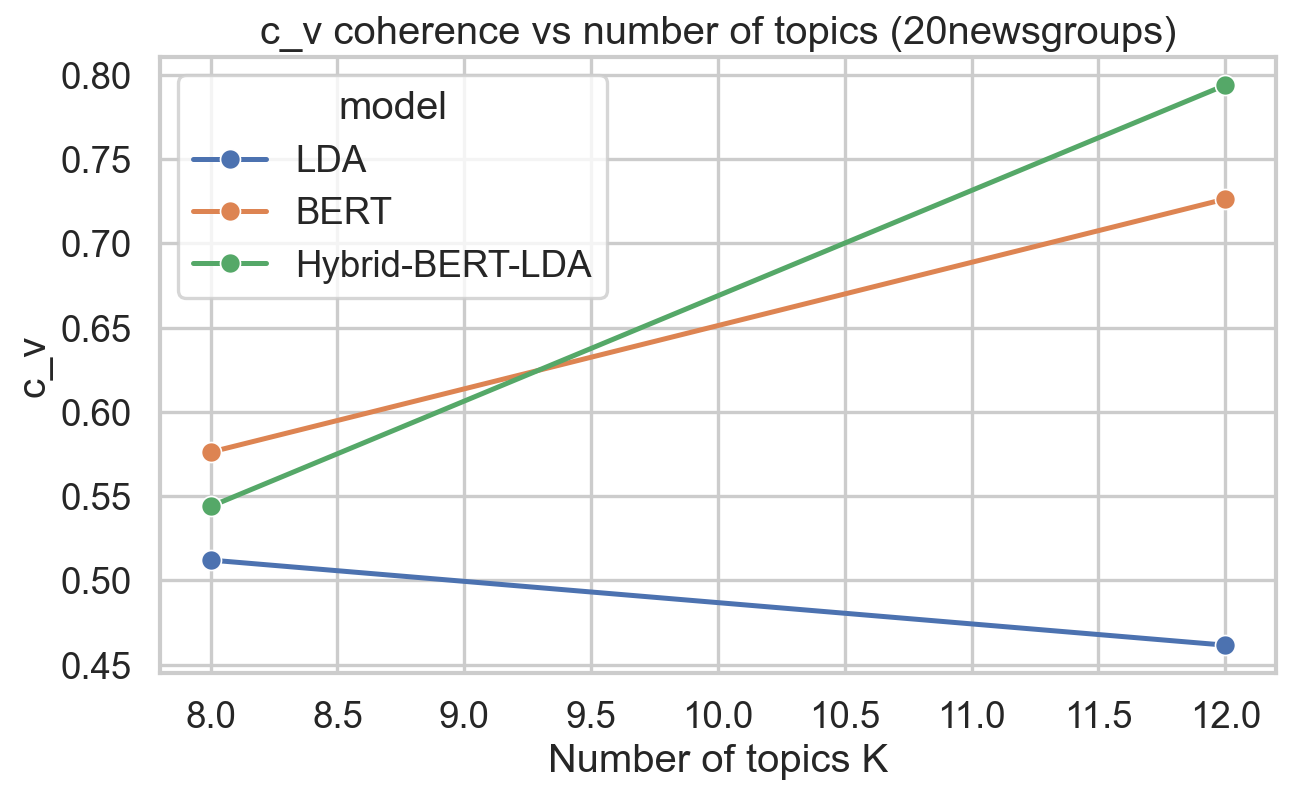
\includegraphics[width=\linewidth]{results/figures/coherence_c_v_20newsgroups.png}
  \caption{20 Newsgroups}
\end{subfigure}\hfill
\begin{subfigure}[t]{0.48\textwidth}
  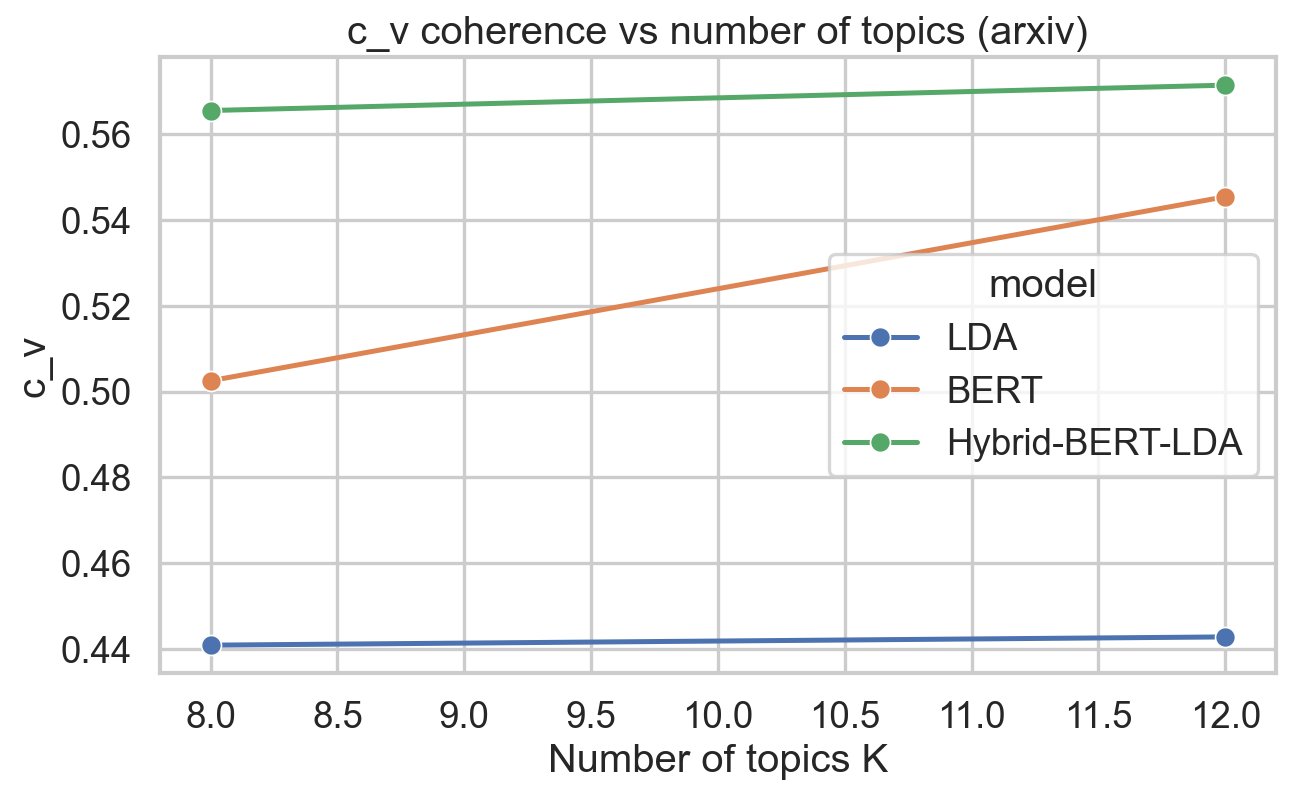
\includegraphics[width=\linewidth]{results/figures/coherence_c_v_arxiv.png}
  \caption{arXiv}
\end{subfigure}
\caption{$C_v$ as a function of the number of topics $K$.}
\label{fig:cv}
\end{figure}

\begin{figure}[htbp]
\centering
\begin{subfigure}[t]{0.48\textwidth}
  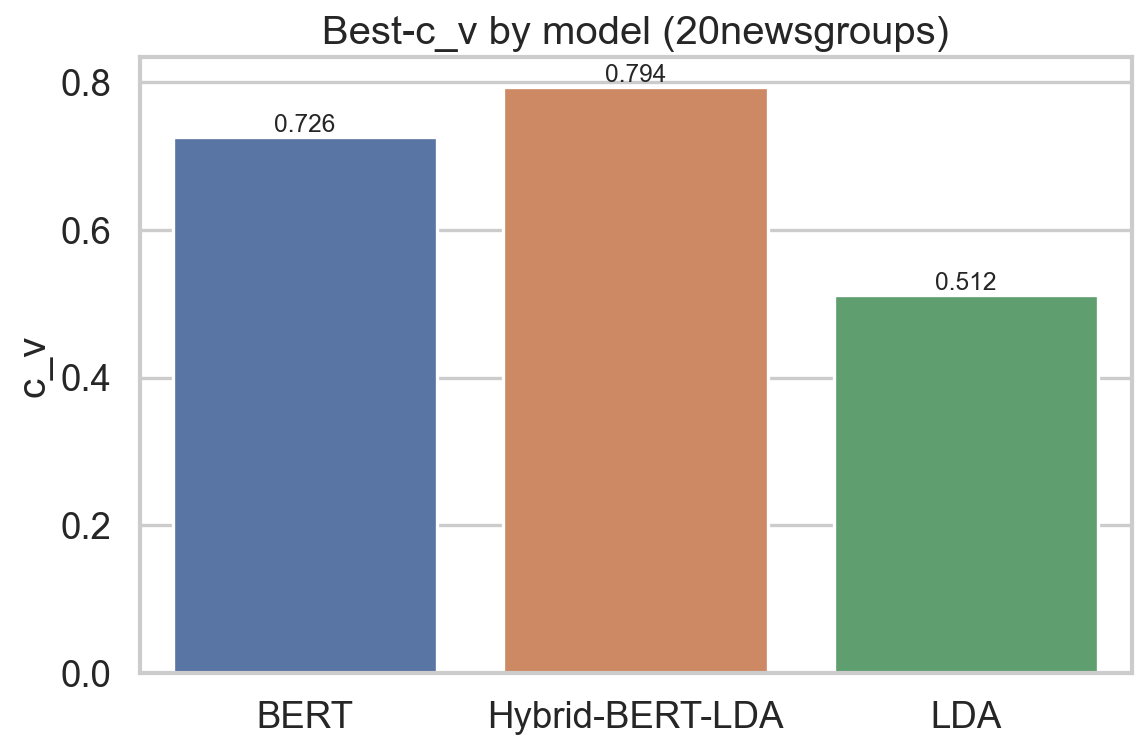
\includegraphics[width=\linewidth]{results/figures/best_c_v_20newsgroups.png}
  \caption{20 Newsgroups}
\end{subfigure}\hfill
\begin{subfigure}[t]{0.48\textwidth}
  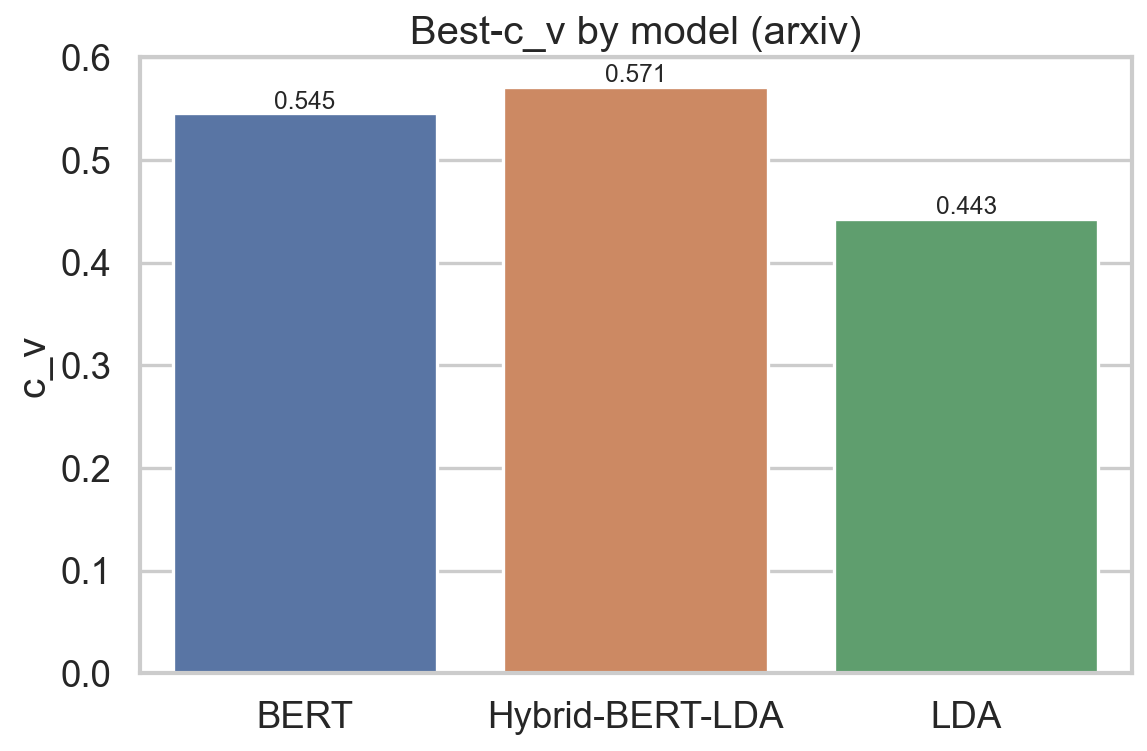
\includegraphics[width=\linewidth]{results/figures/best_c_v_arxiv.png}
  \caption{arXiv}
\end{subfigure}
\caption{Best $C_v$ attained by each model.}
\label{fig:best}
\end{figure}

Paul et al.~\cite{paul2025} observed a smaller absolute gain ($0.63$ to $0.66$). The larger movement here is not directly comparable, because the hybrid topics are c-TF-IDF lists from embedding-informed clusters rather than LDA's own $\phi_k$. The comparison that the design cares about is still LDA versus hybrid on the same corpus and the same coherence function, and that comparison favours the hybrid in both collections.

\subsection{Choice of $\alpha$}
Table~\ref{tab:alpha} and Figure~\ref{fig:alpha} show $C_v$ as $\alpha$ varies at the hybrid's preferred $K$. On 20~Newsgroups the peak is at $\alpha=0.5$. On arXiv it is at $\alpha=0.25$: a smaller LDA component and a larger embedding component. Setting $\alpha=1$, which discards the embedding, is the weakest setting on arXiv. Concatenation is therefore not treated as a single recipe; the mix is chosen on the same metric used to compare against LDA.

\begin{table}[htbp]
\centering
\caption{$C_v$ while sweeping the LDA weight $\alpha$ at the best $K$.}
\label{tab:alpha}
\small
\begin{tabular}{@{}lccccc@{}}
\toprule
Corpus & $\alpha=0$ & $0.25$ & $0.5$ & $0.75$ & $1.0$ \\
\midrule
20 Newsgroups ($K=12$) & 0.67 & 0.57 & 0.79 & 0.68 & 0.60 \\
arXiv ($K=12$) & 0.67 & 0.72 & 0.57 & 0.55 & 0.49 \\
\bottomrule
\end{tabular}
\end{table}

\begin{figure}[htbp]
\centering
\begin{subfigure}[t]{0.48\textwidth}
  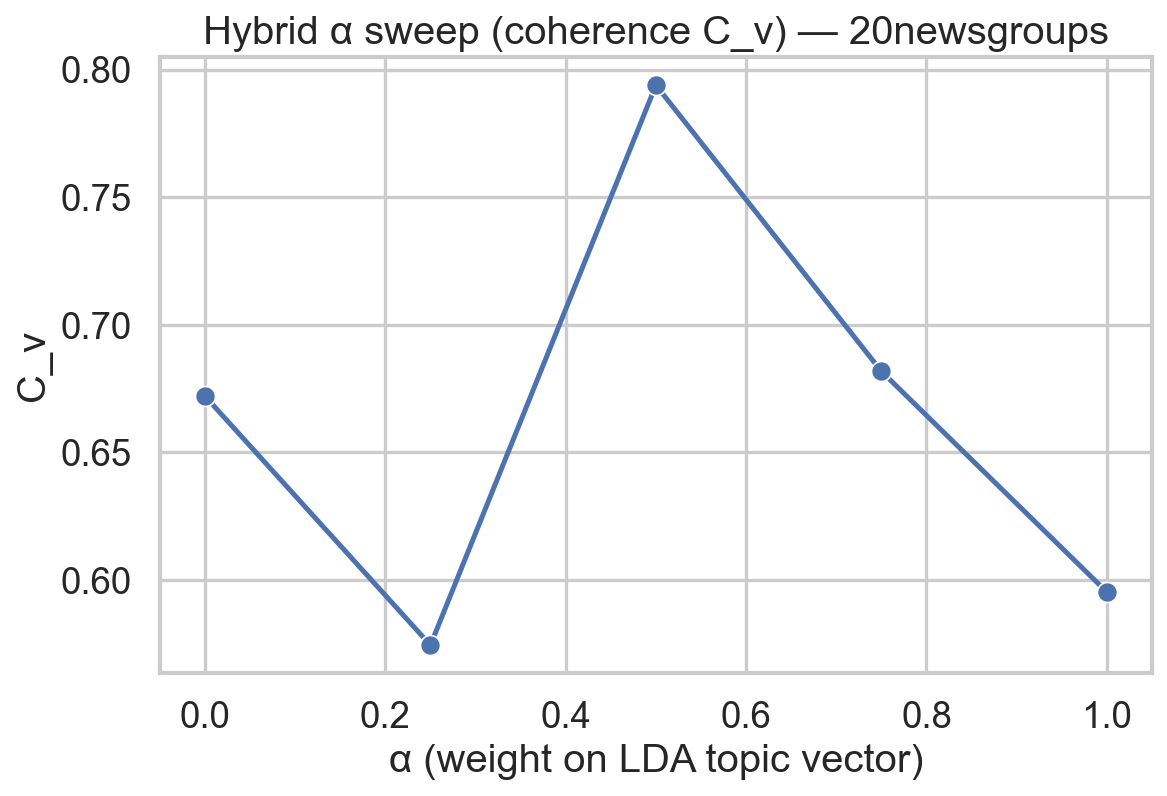
\includegraphics[width=\linewidth]{results/figures/alpha_sweep_20newsgroups.png}
  \caption{20 Newsgroups}
\end{subfigure}\hfill
\begin{subfigure}[t]{0.48\textwidth}
  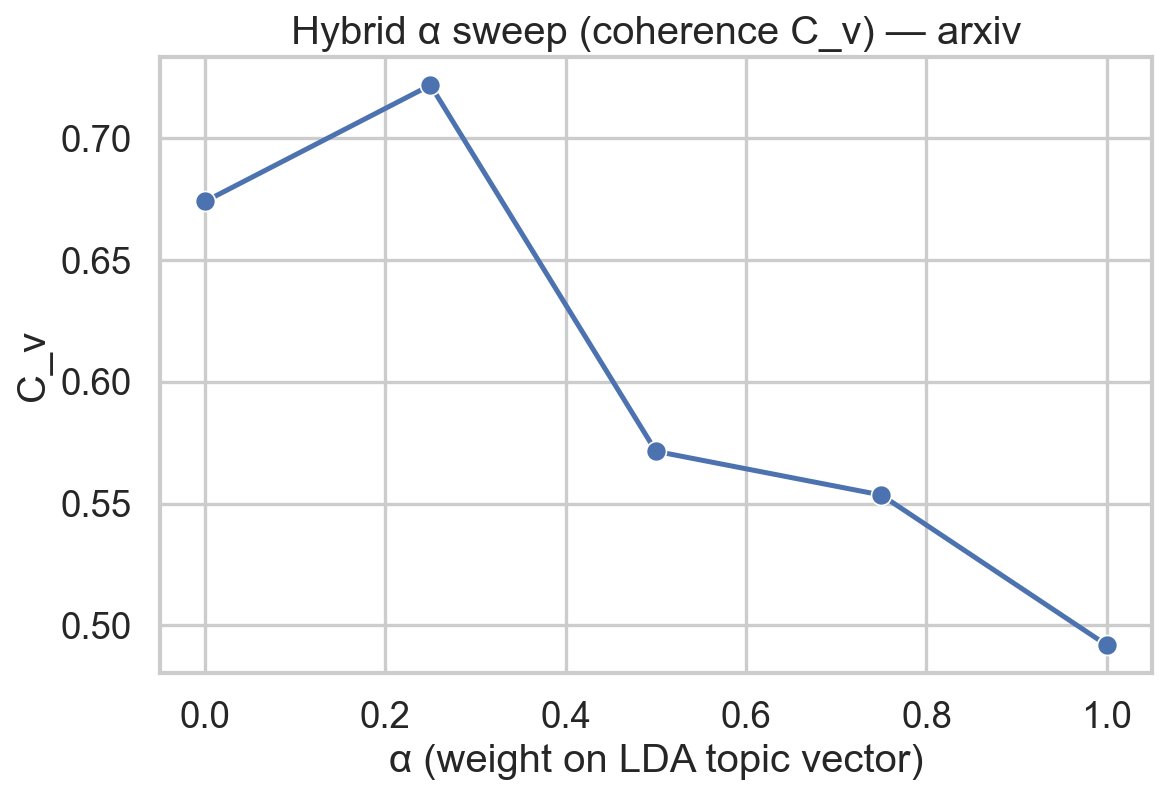
\includegraphics[width=\linewidth]{results/figures/alpha_sweep_arxiv.png}
  \caption{arXiv}
\end{subfigure}
\caption{$C_v$ against the concatenation weight $\alpha$.}
\label{fig:alpha}
\end{figure}

\subsection{Silhouette after PCA, t-SNE and UMAP}
Table~\ref{tab:sil} and Figure~\ref{fig:sil} repeat the reducer comparison from~\cite{george2023}. UMAP gives the highest silhouette for every model. LDA can look strong on this metric because $\theta$ is already low-dimensional; a neat clustering of topic proportions does not imply that the associated word lists are coherent. That is why $C_v$ is the figure of merit in Table~\ref{tab:cv} and silhouette is kept as a secondary check.

\begin{table}[htbp]
\centering
\caption{Silhouette coefficients at $K=12$.}
\label{tab:sil}
\small
\begin{tabular}{@{}llccc@{}}
\toprule
Corpus & Model & PCA & t-SNE & UMAP \\
\midrule
20 Newsgroups & LDA & 0.29 & 0.49 & 0.59 \\
20 Newsgroups & BERT & 0.13 & 0.41 & 0.44 \\
20 Newsgroups & Hybrid & 0.22 & 0.48 & 0.53 \\
arXiv & LDA & 0.24 & 0.43 & 0.50 \\
arXiv & BERT & 0.10 & 0.36 & 0.37 \\
arXiv & Hybrid & 0.18 & 0.42 & 0.45 \\
\bottomrule
\end{tabular}
\end{table}

\begin{figure}[htbp]
\centering
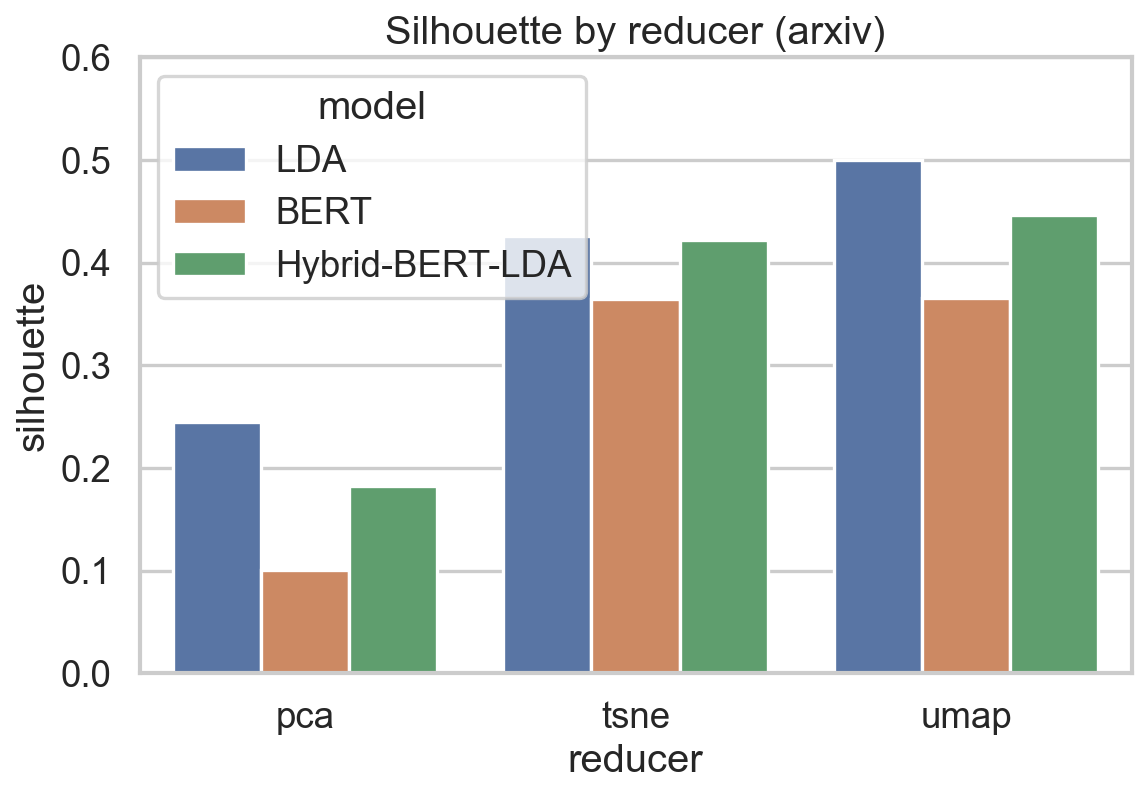
\includegraphics[width=0.72\textwidth]{results/figures/silhouette_arxiv.png}
\caption{Silhouette on arXiv for PCA, t-SNE and UMAP.}
\label{fig:sil}
\end{figure}

\subsection{Topic words}
LDA's arXiv topics tend to reuse generic terms such as \texttt{model}, \texttt{network} and \texttt{algorithm}. The hybrid lists are not perfect, but they more often line up with named research themes. Table~\ref{tab:words} gives a few examples from the $K=12$ arXiv run.

\begin{table}[htbp]
\centering
\caption{Selected hybrid clusters on arXiv ($K=12$), labelled by hand from the top words.}
\label{tab:words}
\small
\begin{tabular}{@{}clp{9.6cm}@{}}
\toprule
ID & Theme & Top words \\
\midrule
3 & Adversarial learning & attack, backdoor, adversarial, privacy, defense, trigger \\
4 & Large language models & llm, language, prompt, reasoning, question, knowledge \\
6 & Vision and language & video, vlms, caption, grounding, spatial, visual \\
8 & Reinforcement learning & learning, bound, reinforcement, optimization, mdp \\
9 & Graph learning & graph, node, clustering, subgraphs, vertex \\
11 & Medical imaging & nodule, lung, cancer, segmentation, infection \\
\bottomrule
\end{tabular}
\end{table}

\subsection{Dashboard}
The Streamlit application reads the files written by the pipeline and exposes the same quantities interactively: coherence charts, side-by-side LDA and hybrid word lists, the UMAP scatter, the yearly prevalence plot, and a text box that returns nearest abstracts for a pasted query. It is intended as a viewer for the fitted models rather than as a second training procedure.

\subsection{Geometry and time}
Figure~\ref{fig:umap} shows a two-dimensional UMAP of the hybrid vectors, coloured by $k$-means assignment. Well separated regions correspond to distinct themes; overlap is expected for papers that sit between areas. Figure~\ref{fig:temporal} plots mean $\theta$ by year for the arXiv sample, which contains between 45 and 56 abstracts in each year from 2018 to 2025. 20~Newsgroups has no dates, so the temporal plot is arXiv only.

\begin{figure}[htbp]
\centering
\begin{subfigure}[t]{0.48\textwidth}
  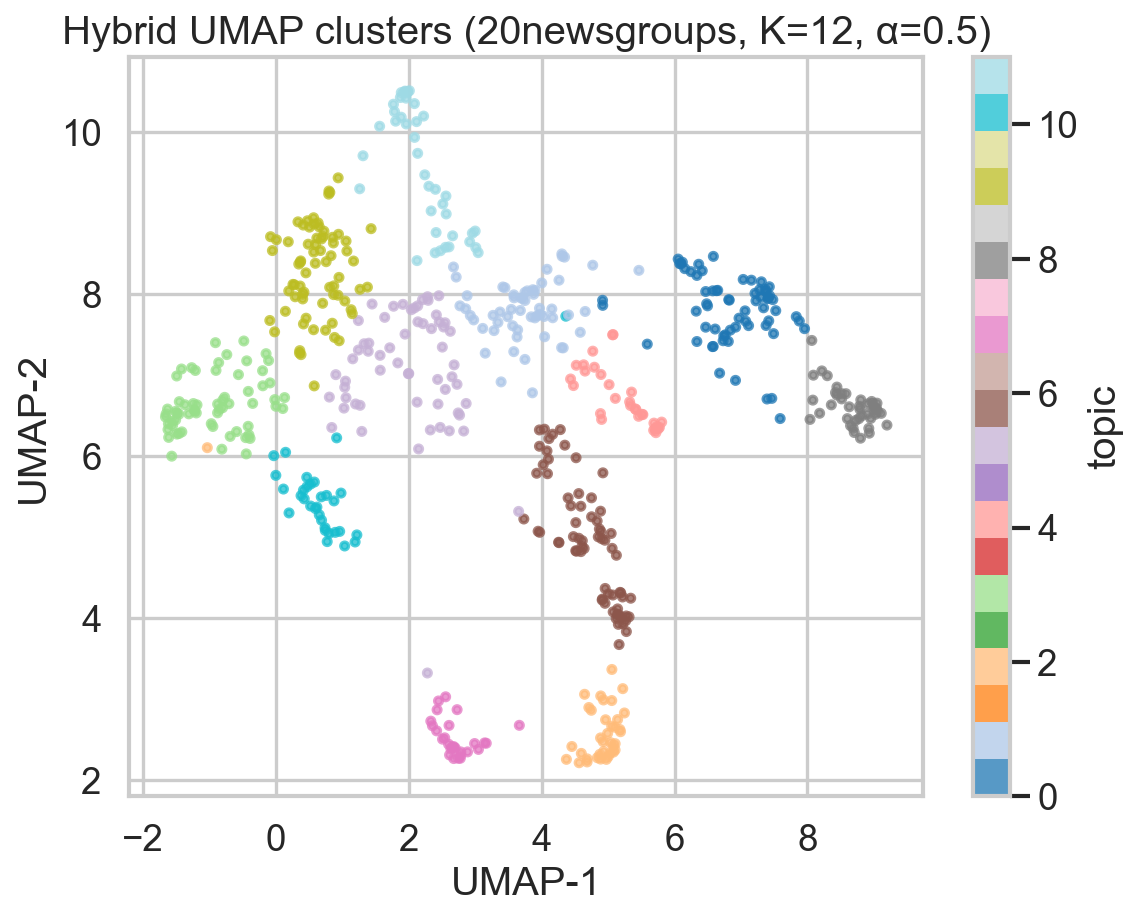
\includegraphics[width=\linewidth]{results/figures/umap_20newsgroups.png}
  \caption{20 Newsgroups}
\end{subfigure}\hfill
\begin{subfigure}[t]{0.48\textwidth}
  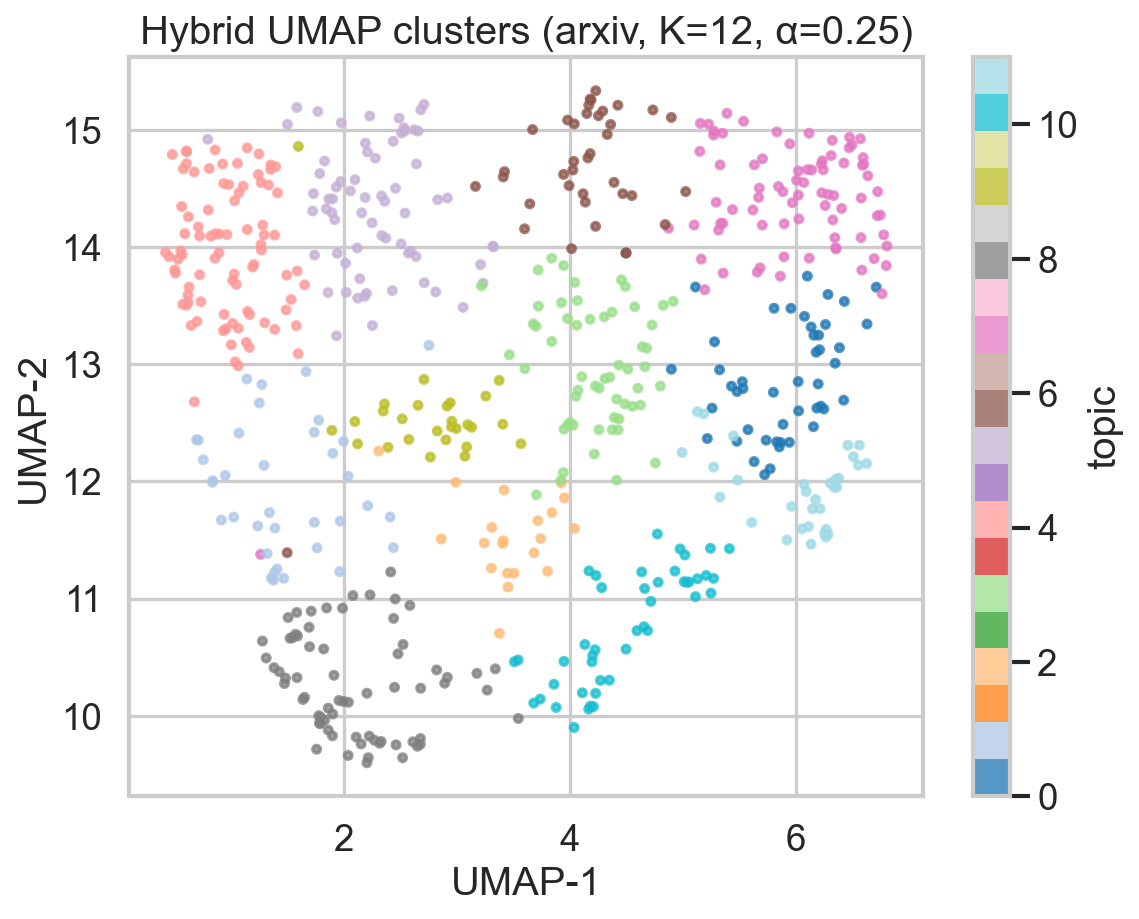
\includegraphics[width=\linewidth]{results/figures/umap_arxiv.png}
  \caption{arXiv}
\end{subfigure}
\caption{UMAP of hybrid document vectors, coloured by cluster.}
\label{fig:umap}
\end{figure}

\begin{figure}[htbp]
\centering
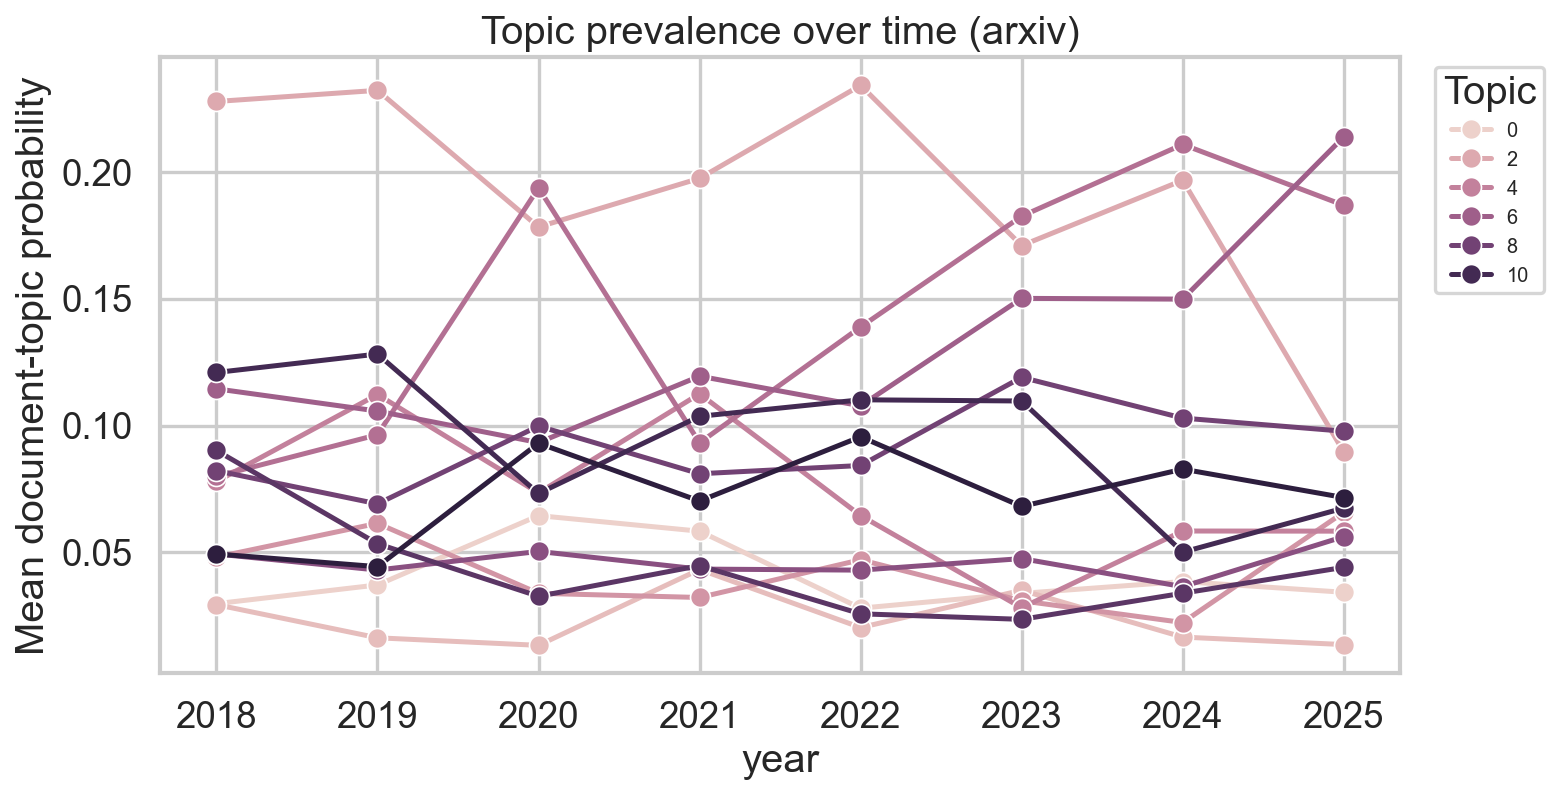
\includegraphics[width=0.88\textwidth]{results/figures/temporal_arxiv.png}
\caption{Mean document--topic probability on arXiv by year of publication.}
\label{fig:temporal}
\end{figure}

\section{Discussion}
\label{sec:discuss}

Table~\ref{tab:compare} places this prototype next to the two papers it was built from. The concatenation-and-cluster pattern is the same. What differs is the evaluation on scientific text with $C_v$ against LDA, the search over $\alpha$, the use of publication years, and a retrieval interface.

\begin{table}[htbp]
\centering
\caption{Coverage relative to the two source papers.}
\label{tab:compare}
\small
\begin{tabular}{@{}p{3.5cm}p{3.5cm}p{3.5cm}p{3.5cm}@{}}
\toprule
 & Paul et al.~\cite{paul2025} & George \& Sumathy~\cite{george2023} & This work \\
\midrule
LDA + BERT concat & yes & yes & yes \\
$C_v$ versus LDA & news; $+0.03$ & no (silhouette) & arXiv; up to $+0.28$ \\
Scientific corpus & 20~Newsgroups extra & CORD-19 & arXiv with years \\
UMAP + $k$-means & clustering & yes & yes \\
$\alpha$ selected on $C_v$ & not reported & not reported & $\alpha=0.25$ on arXiv \\
Topics over time & no & no & 2018--2025 \\
Related-work query & no & no & dashboard \\
\bottomrule
\end{tabular}
\end{table}

A plausible account of the coherence gain is as follows. LDA estimates a global co-occurrence structure and, as a by-product, an interpretable $\theta_d$. Sentence-BERT estimates local similarity, including paraphrases that never share a context window in this corpus. Putting the two in one vector lets $k$-means split documents that LDA would have mixed because they share function words. Class-based TF-IDF then names the split. $C_v$ tests those names, which is closer to what a reader sees than a silhouette in embedding space.

Several limits should be kept in mind. Six hundred abstracts per corpus is a convenience sample, not a substitute for tens of thousands of papers. MiniLM was trained on general web text; a scientific encoder would be a fairer semantic model for arXiv. No intruder-word study was run, so the human side of interpretability is informal. Yearly averages of $\theta$ assume that the topics themselves do not drift, which is a strong assumption if the goal is a full dynamic analysis~\cite{blei2006}.

\section{Conclusion}
\label{sec:end}

LDA already gives a probabilistic description of a corpus. The question asked here is whether a frozen sentence embedding, concatenated with that description and clustered, produces word lists that cohere better than LDA's own topics. In the experiments it does. On 20~Newsgroups the best hybrid $C_v$ is $0.79$ against $0.51$ for LDA. On arXiv abstracts from 2018--2025 the corresponding comparison is $0.44$ for LDA against $0.57$ at $\alpha=0.5$ and $0.72$ at $\alpha=0.25$. Silhouette scores, an $\alpha$ curve, a temporal plot and a small retrieval interface sit around that comparison. The generative model is not discarded; it is used as one view of the document, and the embedding is used as the other.

\clearpage
\begin{thebibliography}{11}

\bibitem{blei2003}
D.~M. Blei, A.~Y. Ng, and M.~I. Jordan,
``Latent Dirichlet allocation,''
\emph{Journal of Machine Learning Research}, vol.~3, pp.~993--1022, 2003.

\bibitem{blei2006}
D.~M. Blei and J.~D. Lafferty,
``Dynamic topic models,''
in \emph{Proc.\ ICML}, 2006, pp.~113--120.

\bibitem{devlin2019}
J.~Devlin, M.-W. Chang, K.~Lee, and K.~Toutanova,
``BERT: Pre-training of deep bidirectional transformers for language understanding,''
in \emph{Proc.\ NAACL-HLT}, 2019, pp.~4171--4186.

\bibitem{reimers2019}
N.~Reimers and I.~Gurevych,
``Sentence-BERT: Sentence embeddings using Siamese BERT-networks,''
in \emph{Proc.\ EMNLP-IJCNLP}, 2019, pp.~3982--3992.

\bibitem{paul2025}
P.~C. Paul, M.~Rahman, A.~Begum, M.~T. Ahmed, D.~Chakraborty, and M.~S. Rahman,
``Combining BERT with LDA: Improved topic modeling in Bengali language,''
\emph{IAENG International Journal of Computer Science}, vol.~52, no.~2, pp.~383--393, 2025.

\bibitem{george2023}
L.~George and P.~Sumathy,
``An integrated clustering and BERT framework for improved topic modeling,''
\emph{International Journal of Information Technology}, vol.~15, pp.~2187--2195, 2023.

\bibitem{beltagy2019}
I.~Beltagy, K.~Lo, and A.~Cohan,
``SciBERT: A pretrained language model for scientific text,''
in \emph{Proc.\ EMNLP-IJCNLP}, 2019, pp.~3615--3620.

\bibitem{grootendorst2022}
M.~Grootendorst,
``BERTopic: Neural topic modeling with a class-based TF-IDF procedure,''
arXiv:2203.05794, 2022.

\bibitem{roder2015}
M.~R\"oder, A.~Both, and A.~Hinneburg,
``Exploring the space of topic coherence measures,''
in \emph{Proc.\ WSDM}, 2015, pp.~399--408.

\bibitem{mcinnes2018}
L.~McInnes, J.~Healy, and J.~Melville,
``UMAP: Uniform manifold approximation and projection for dimension reduction,''
arXiv:1802.03426, 2018.

\bibitem{xie2020}
Q.~Xie, X.~Zhang, Y.~Ding, and M.~Song,
``Monolingual and multilingual topic analysis using LDA and BERT embeddings,''
\emph{Journal of Informetrics}, vol.~14, no.~3, 2020.

\end{thebibliography}

\end{document}
